
\section{Improved Metropolis Hasting for Bayesian Inference using FFBS  within the Gibbs Sampling On MJPs}~
\setlength{\unitlength}{0.8cm}
  \begin{figure}[H]
  \centering
  \begin{minipage}[!hp]{0.45\linewidth}
  \centering
    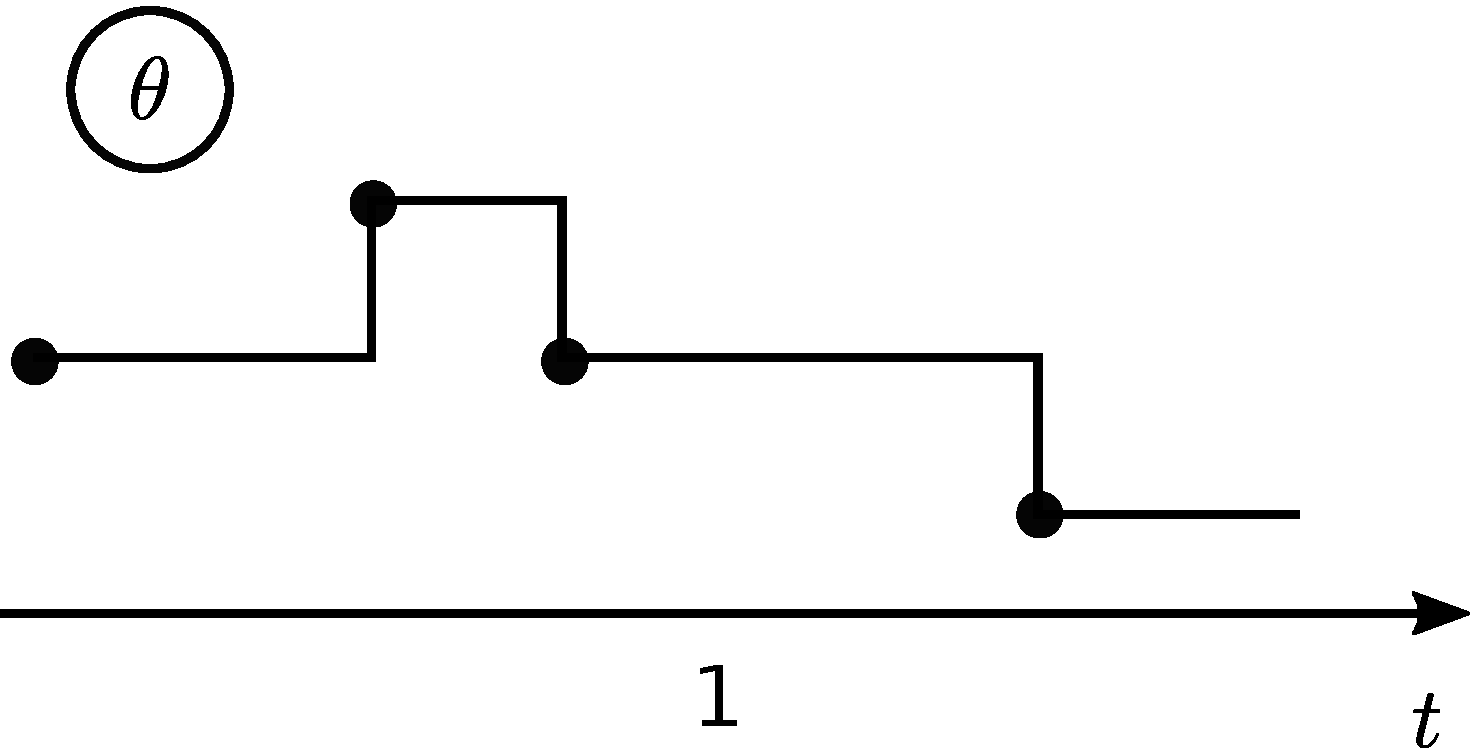
\includegraphics [width=0.70\textwidth, angle=0]{figs/plot0.pdf}
      \end{minipage}
  \begin{minipage}[hp]{0.45\linewidth}
  \centering
    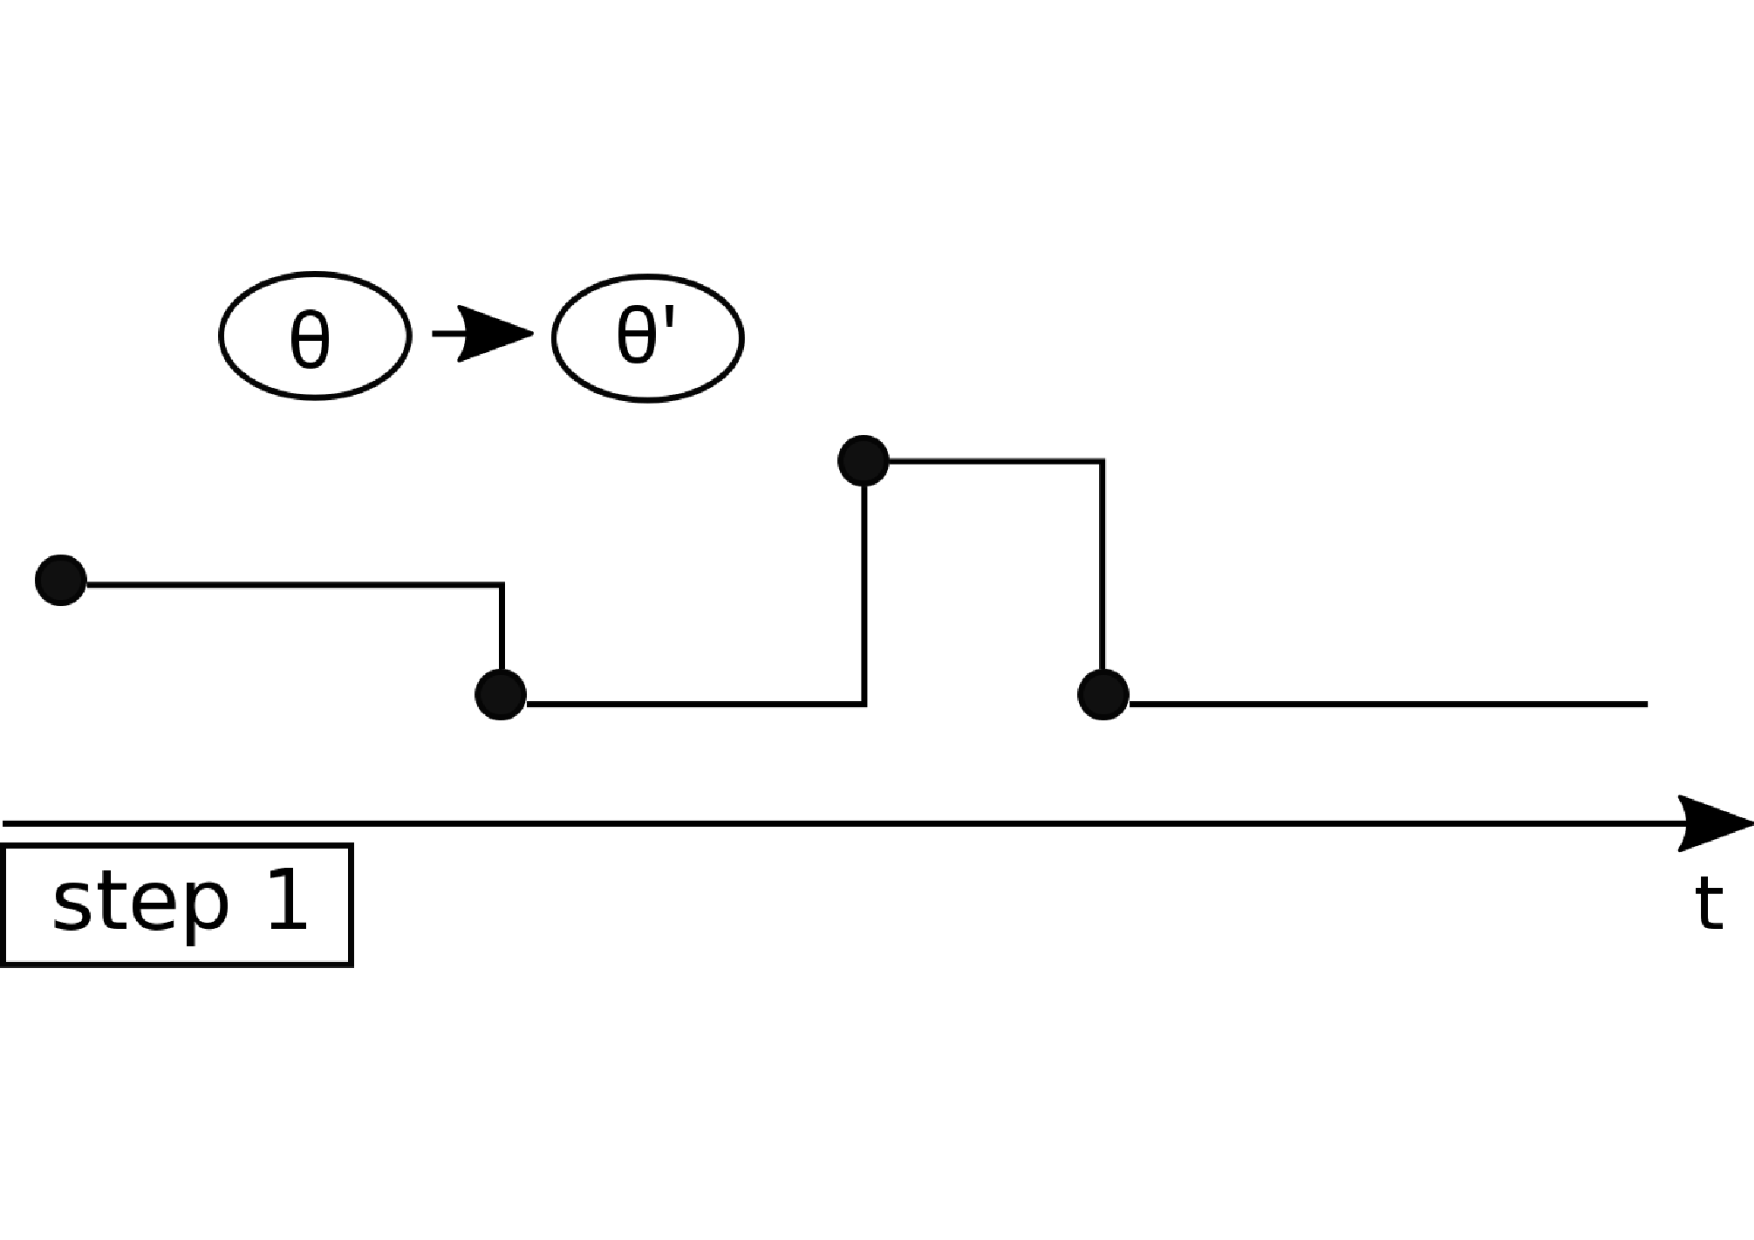
\includegraphics [width=0.70\textwidth, angle=0]{figs/plot1.pdf}
    \vspace{-0 in}
  \end{minipage}
  \begin{minipage}[hp]{0.45\linewidth}
  \centering
    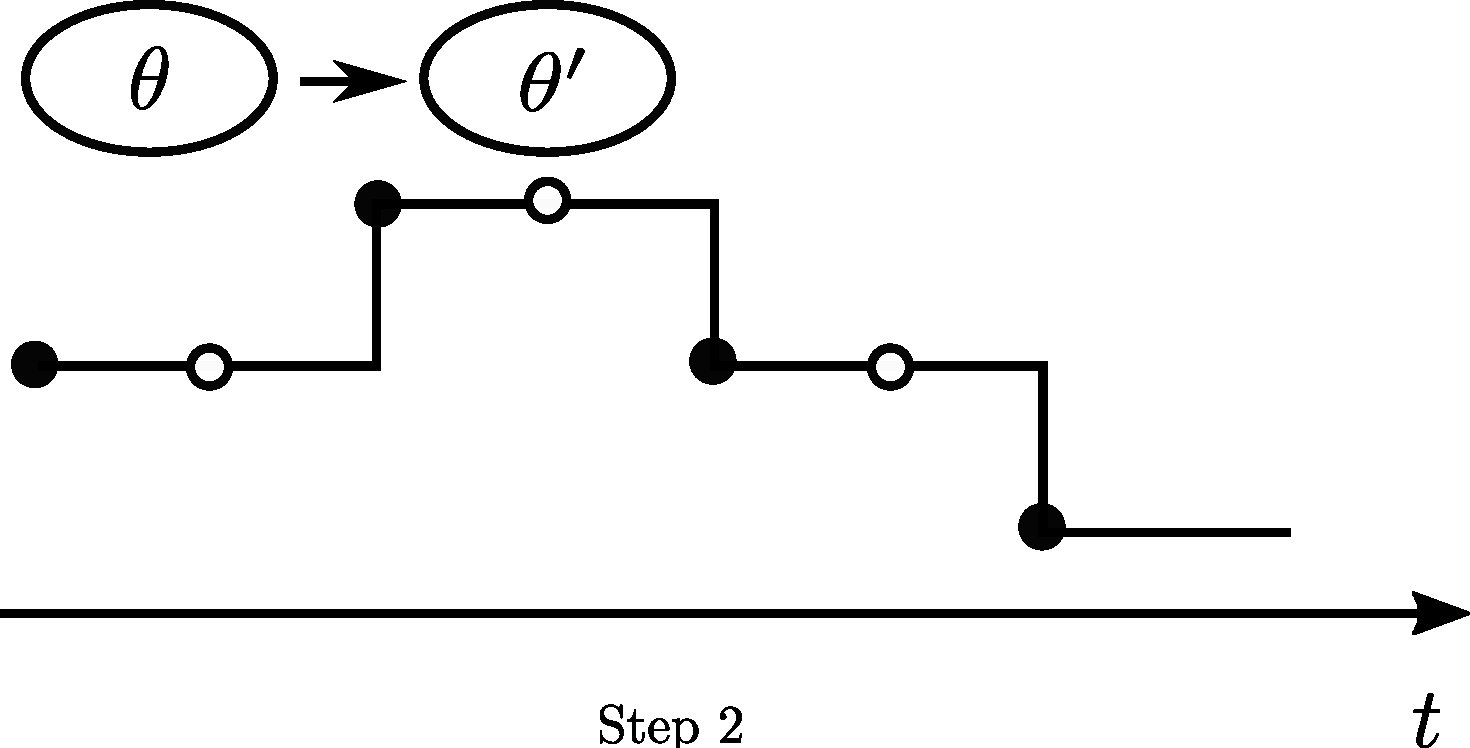
\includegraphics [width=0.70\textwidth, angle=0]{figs/plot2.pdf}
    \vspace{-0 in}
  \end{minipage}
  \begin{minipage}[hp]{0.45\linewidth}
  \centering
    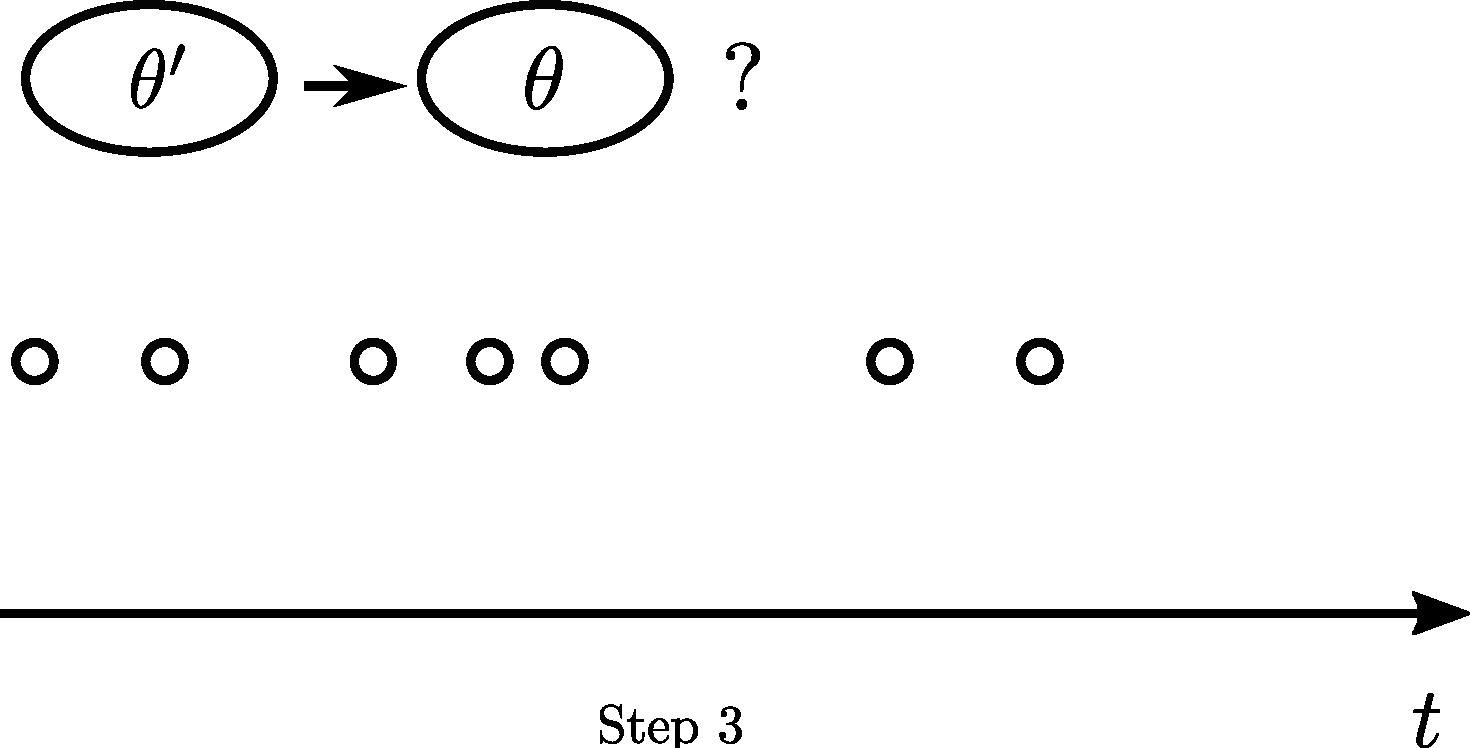
\includegraphics [width=0.70\textwidth, angle=0]{figs/plot3.pdf}
    \vspace{-0 in}
  \end{minipage}
  \begin{minipage}[hp]{0.45\linewidth}
  \centering
    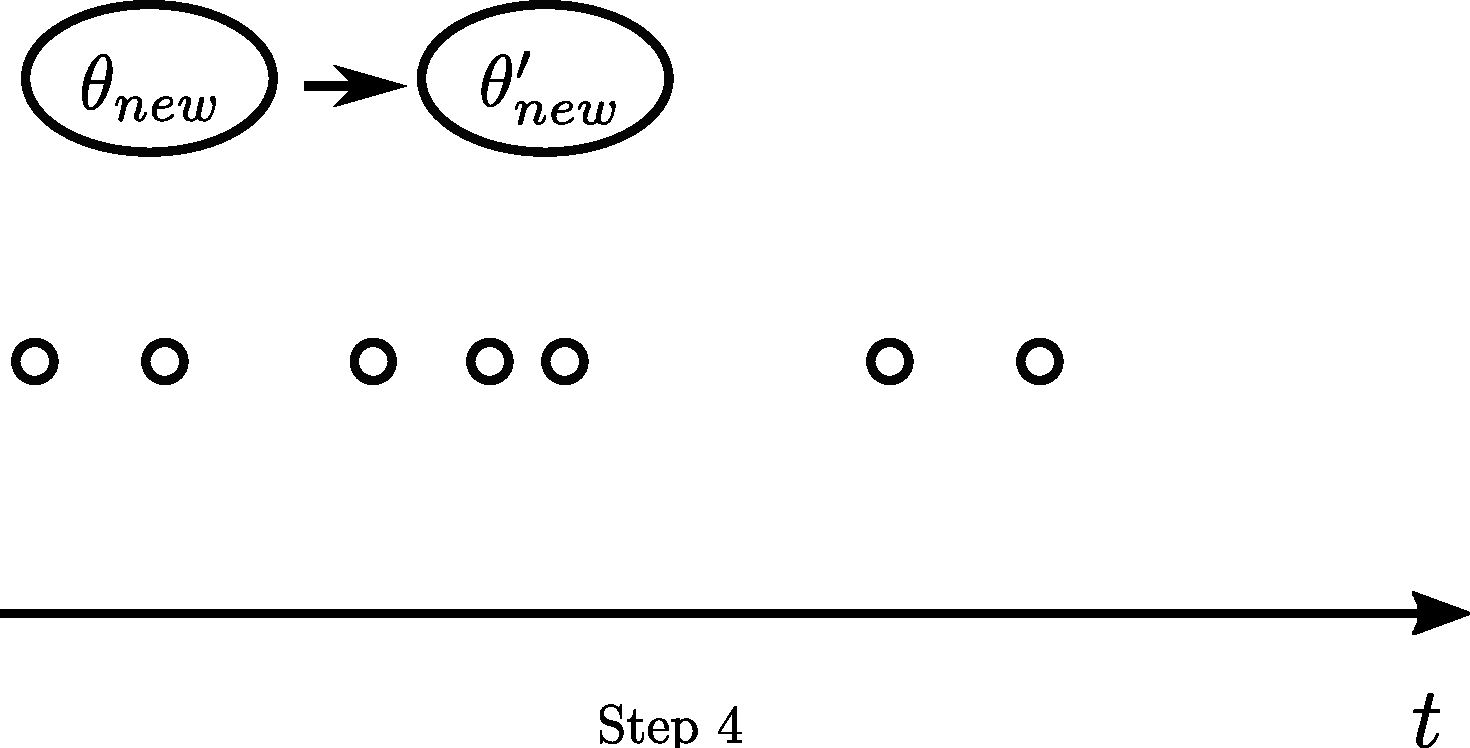
\includegraphics [width=0.70\textwidth, angle=0]{figs/plot4.pdf}
    \vspace{-0 in}
  \end{minipage}
  \begin{minipage}[hp]{0.45\linewidth}
  \centering
    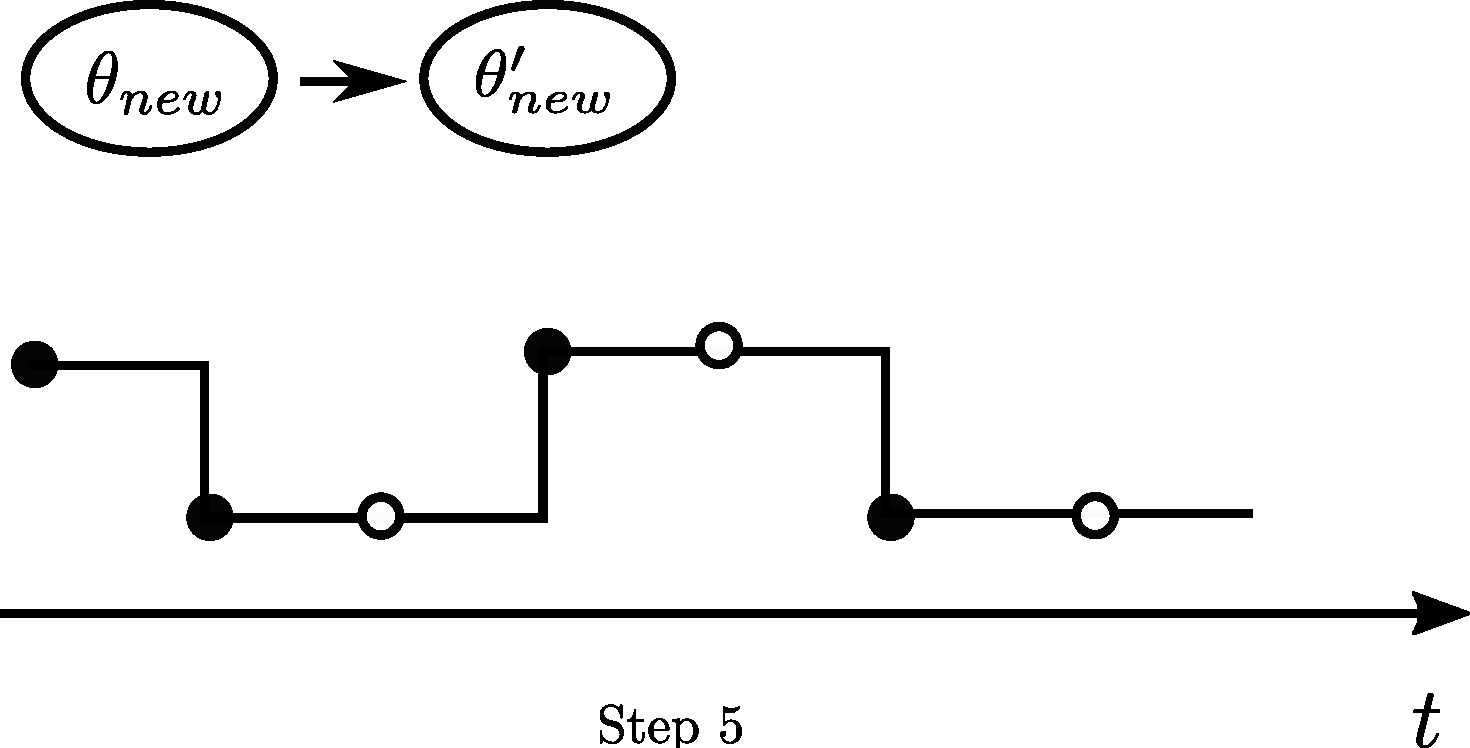
\includegraphics [width=0.70\textwidth, angle=0]{figs/plot5.pdf}
    \vspace{-0 in}
  \end{minipage}
  \begin{minipage}[hp]{0.45\linewidth}
  \centering
    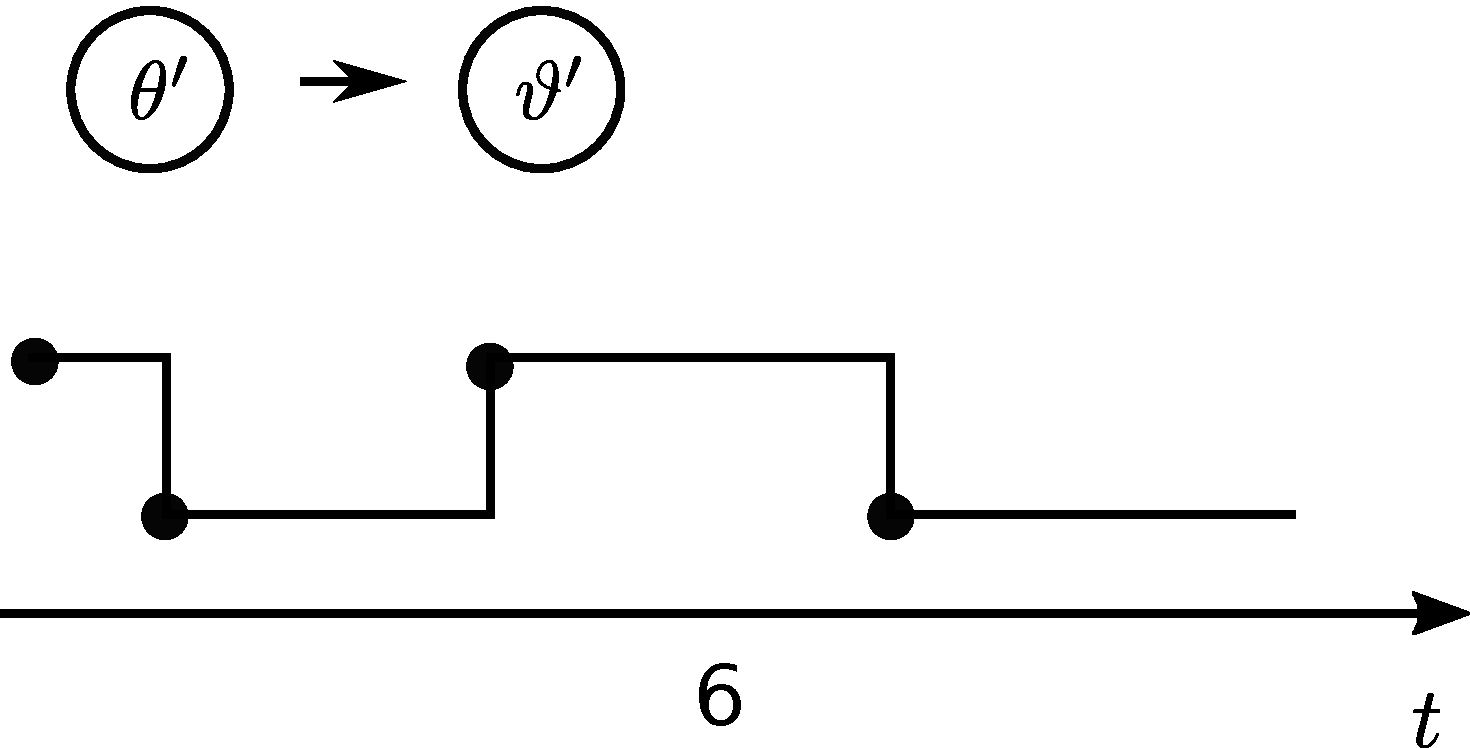
\includegraphics [width=0.70\textwidth, angle=0]{figs/plot6.pdf}
    \vspace{-0 in}
  \end{minipage}

    \caption{Improved MH algorithm}

  \end{figure}

\begin{algorithm}[H]
   \caption{MH In Gibbs sampling for MJPs }
   \label{alg:MH In Gibbs}
\begin{algorithmic}
   \State {\bfseries Input:} A set of partial and noisy observations $y_{[t_0, t_{N+1})}$, Initial distribution over states $\pi_0$,  Metropolis Hasting proposal $q(. | \theta)$.\\
   The previous MJP path $S(t) = (S, T)$, the previous MJP parameters $(\theta)$.\\  
      \State {\bfseries Output:} A new MJP trajectorie $\tilde{S} (t) = (\tilde{S}, \tilde{T})$, A series of MJP parameters $\tilde{\theta}$.
      \State 0:  Sample $\theta^* \sim q(.| \theta)$. And let $\Omega = h(\theta) + h(\theta^*)$, with $h(\theta) > max_s{|A_s(\theta)|}$, $h(\theta^*) > max_s{|A_s(\theta^*)|}$ using some deterministic function $h$.
    \State 1: Sample virtual jumps $U\subset[t_{start}, t_{end}]$ from a Non homogeneous Poisson process with piecewise-constant rate$$R(t) = (\Omega + A_{S(t)}(\theta)).$$\\Define $W = T \cup U$.
    \State 2: Propose $(\theta^*, \theta)$ and accept $\theta^*$ as $\tilde{\theta}$ with probability $\alpha$.
        \begin{align*}
        \alpha &=  1 \wedge \frac{P(W,(\theta^*, \theta)| y)}{P(W, (\theta, \theta^*)| y)}\\
        &=  1 \wedge \frac{P(y| W,\theta^*, \theta) P(W | (\theta^*, \theta))p((\theta^*, \theta))}{P(y| W,(\theta, \theta^*)) P(W | (\theta, \theta^*))p((\theta, \theta^*))}\\
                &=  1 \wedge \frac{P(y| W,\theta^*, \theta)p((\theta^*, \theta))}{P(y| W,(\theta, \theta^*))p((\theta, \theta^*))}.
        \end{align*}
    \State 3: Sample a path $\tilde{V}$, from a discret-time Markov chain with $|W| + 1$ steps, using FFBS algorithm. The transition matrix of the Markov chain is $B = (I + \frac{A(\tilde{\theta})}{\Omega})$ while the initial distribution over states is $\pi_0$. The likelihood of state $s$ at step $i$ is 
    $$ L_i(s) = P(Y_{[w_i, w_{i + 1})} | S(t) = s \; for\; t \in [w_i, w_{i + 1})) = \prod_{j: t_j \in [w_i, w_{i + 1})}p(y_{t_j} | S(t_j) = s).$$\\
%(i.e. $V(i) \sim P(V |  \theta(i), W(i - 1), y).$) Then delete all the virtual jumps to get $S(i), T(i) .$\\
    \State 4: Let $\tilde{T}$ be the set of times in $W$ when the Markov chain changes state. Define $\tilde{S}$ as the corresponding set of state values. Return $(\tilde{S}, \tilde{T}, \tilde{\theta})$.\\
\end{algorithmic}
\end{algorithm}

To address the limitations of the previous algorithm, we describe
a more efficient scheme. This forms the main contribution of this paper.

Let the current state of the Markov chain be $S(t), \theta$. For some
distribution $q(\theta^*|\theta)$, generate a new parameter
$\theta^*$. Treat this as an auxiliary variable, so that the augmented
space now is the triplet $(S(t), \theta^*,\theta)$. Now, we discard
state information, keeping on the skeleton of transition times.
We now pretend generative process involved a uniformization scheme
where the bounding rate is given by $\Omega(\theta) + \Omega(\theta^*)$.
We can then sample the set of thinned events from a piecewise-constant
Poisson process with intenstity $\Omega(\theta) + \Omega(\theta^*) - 
A_{S(t)}$. Finally, we propose swapping the original parameter
$\theta$ with the auxiliary parameter $\theta^*$. Observe that the
skeleton of Poisson events $T \cup U$ has the same probability both
before and after this proposal, so that unlike the previous scheme,
the term does not affect the acceptance proposal. Instead, the output
probability depends only on the probability of the observations
under both set of parameters, as we can use the forward-backward algorithm
to integrate out MJP state spaces. Thus our acceptance probability is
just given by
$$ \text{acc} = 
  \min\left(1, \frac{p(X,\theta^*)q(\theta|\theta^*)}
   {p(X,\theta)q(\theta^*|\theta)}\right) = 
  \min\left(1, \frac{p(X|\theta^*)p(\theta^*)q(\theta|\theta^*)}
   {p(X|\theta)p(\theta)q(\theta^*|\theta)}\right)
   $$.
   The terms $p(X|\theta^*)$ and  $p(X|\theta)$ can be calculated by 
   running a forward pass of the forward-backward algorithm. Having
   accepted or rejected the proposal, a new trajectory is sampled by
   completing the backward pass.
